\chapter{Implementierung}
\label{implementierung}
Die Umsetzung der zu Beginn genannten Funktionalitäten wird innerhalb der folgenden Teilabschnitte beschrieben. Der erste Teilabschnitt dieses Kapitels dokumentiert die entwickelte Software \cite{badps2}, welche den Mikrocontroller steuert und den Programmablauf der einzelnen Funktionalitäten zeigt. Eine detaillierte Darstellung der implementierten Software befindet sich zudem in dem Abschnitt \ref{source_code} des Anhangs und auf der beigelegten CD-ROM. Der zweite Teil dieses Kapitels erläutert den Aufbau der Elektronik und zeigt wie die verwendete Hardware mit dem Mikrocontroller zusammengebaut wurde.



\section{Softwaredokumentation}
Die implementierten Softwarekomponenten \cite{badps2} gliedern sich in die drei Abschnitte für die jeweiligen Funktionalitäten, die Aufnahme von Tastatureingaben, die Wiedergabe von Tastatureingaben mittels SD-Karte und die Wiedergabe von Tastatureingaben über Ethernet. Diese beinhalten Hilfsfunktionen für die Tastatur, für die SD-Karte und für die Webseite, welche vorab in den nächsten Abschnitten beschrieben werden. Abschließend wird der gesamte Programmablauf beschrieben, der aus den Standardfunktionen des Arduino Mikrocontroller besteht und den Wechsel zwischen den Funktionalitäten ermöglicht.



\subsection{Hilfsfunktionen für die Tastatur}
Um die Kommunikation zwischen der Tastatur und dem Mikrocontroller zu gewährleisten werden einige Hilfsfunktionen benötigt, die in den folgenden Teilabschnitten erläutert werden. Implementiert sind Funktionen zur Initialisierung der Tastatur, dem Lesen und Schreiben von Tastatureingaben, dem Senden von Befehlen an die Tastatur und zwei Hilfsfunktionen zur Steuerung der Daten- bzw. Taktleitung. Alle diese Funktionen sind unter Berücksichtigung der Abläufe des PS/2-Protokolls implementiert.

\subsubsection{void setHigh(int pin)}
Diese Hilfsfunktion nimmt eine Pinnummer des Mikrocontrollers entgegen und setzt den Pinmode für diese Nummer auf Input. Zudem wird eine 1 bzw. das Signal High auf die Leitung dieses Pins gelegt. Dies stellt die Funktionsweise eines Pullup Resistors dar und erlaubt somit eine Schaltung ohne Widerstand \cite{arduino_pullup}.

\subsubsection{void setLow(int pin)}
Diese Methode nimmt ebenfalls eine Pinnummer des Mikrocontrollers entegegen, aber setzt den Pinmode für diese Nummer auf Output. Weiterhin wird eine 0 bzw. Low auf die Leitung dieses Pins gelegt.

\subsubsection{void initKeys(int dataPin, int clockPin)}
Mithilfe dieser Funktion wird eine Tastatur initialisiert, wobei die Pinnummer der eingehenden Datenleitung und Taktleitung als Parameter übergeben werden. Zu Beginn werden die Daten- und Taktleitung mithilfe der zuvor beschriebenen Hilfsfunktion setHigh(int pin) auf 1 bzw. High gesetzt. Anschließend wird mit der Hilfsfunktion sendCommand(unsigned char data) der Reset-Befehl 0xff an die Tastatur übermittelt. Da auf diesen Befehl hin ein 0xfa und 0xaa für ein Acknowledge und einen erfolgreichen Reset erwartet werden, wird zweimalig die Hilfsfunktion readKeys(dataPinIn, clockPinIn) aufgerufen, um diese Antworten abzufangen. Abschließend wird eine Nachricht ausgegeben, dass die Tastatur initialisiert ist.

\subsubsection{unsigned char readKeys(int dataPin, int clockPin)}
Diese Methode ermöglicht das Empfangen einer Tasteneingabe über die an den Mikrocontroller angeschlossene Tastatur. Als Parameter werden der Datenpin und der Taktpin des PS/2-Anschlusses entgegen genommen. Da diese Methode dem PS/2-Protokoll folgt, werden beide Pins mit der Methode setHigh(int pin) auf High bzw. 1 gesetzt. Nach einer Verzögerung von 50$\mu$s wird das Fallen der Taktflanke durch eine Schleife abgewartet, womit die Übertragung des Startbits abgewartet wird.

Anschließend folgt eine achtmaliger Schleifendurchlauf für die acht Datenbits, in welchem wieder die fallende Taktflanke durch eine weitere Schleife abgewartet wird. Danach wird das das jeweilige Datenbit entgegen genommen und durch ein logisches Oder mit einem Bit an die richtige Stelle im Ergebnis-Byte gesetzt. Durch einen Linksshift wird das zur Hilfe genommene Bit pro Schleifendurchlauf verschoben.

Nachdem die Daten übertragen wurden, werden sowohl das Paritäts- als auch das Stopbit abgewartet. Dies geschieht ebenfalls mittels Schleifen, welche die Taktflanken abwarten. Abschließend wird die Taktleitung auf Low bzw. 0 gesetzt und die Daten durch das Ergebnis-Byte an die aufrufende Methode zurückgegeben.

\subsubsection{void writeKeys(int dataPin, int clockPin, unsigned char data)}
Durch diese Methode ist es möglich, gemäß dem PS/2-Protokoll eine Tasteneingabe an den Host zu übertragen. Hierfür werden der Datenpin, der Taktpin und ein Datenbyte als Parameter an die Methode übergeben. Zu Beginn werden erst die Datenleitung und dann die Taktleitung durch setLow(int pin) auf Low bzw. 0 gesetzt und nach einer Verzögerung von 50$\mu$s die Taktleitung zurück durch setHigh(int pin) auf High bzw. 1 gesetzt. Mit dieser Befehlsabfolge wird das Startbit an den Host übertragen.

Danach folgt ein achtmaliger Schleifendurchlauf für die acht Datenbits. Innerhalb eines Durchlaufs wird anfangs durch ein logisches Und mit einem Bit geprüft, ob das Datenbit High oder Low ist. Dementsprechend wird mit den bereits erwähnten Hilfsmethoden ein High oder ein Low auf die Datenleitung gesetzt. Anschließend wird die Taktleitung auf Low gesetzt und nach einer Verzögerung von 50$\mu$s die Taktleitung wieder auf High gesetzt. Damit wurde das Datenbit an den Host übertragen. Durch ein exklusives Oder mit dem Datenbit wird im Schleifendurchlauf zudem noch das Paritätsbit gesetzt und das Datenbit selbst danach durch einen Rechtsshift verschoben.

Nachdem die Daten gesendet wurden, wird je nach Zustand des Paritätsbit die Datenleitung auf High oder Low gesetzt und im selben Verlauf wie bisher ein Taktsignal eingeleitet. Dasselbe erfolgt ein weiteres mal für das Stopbit, das durch ein High auf die Datenleitung gesetzt wird.

\subsubsection{void sendCommand(int dataPin, int clockPin, unsigned char data)}
Mithilfe dieser Methode kann der Mikrocontroller einen Befehl an die Tastatur senden, der als Parameter übergeben wird. Gemäß dem PS/2-Protokoll werden zuerst die Daten- und Taktleitung mithilfe der Methode setHigh(int pin) auf High gesetzt. Nach einer Verzögerung von 300$\mu$s wird zuerst die Taktleitung mithilfe von setLow(int pin) auf Low gesetzt und nach einer weiteren Verzögerung von 300$\mu$s die Datenleitung. Die Taktleitung wird dann nach einer Verzögerung von 10$\mu$s mit der bereits genannten Methode auf High gesetzt. Durch diese Abfolge wird der Tastatur, wie in den Grundlagen beschrieben wurde, ein Übertragungswunsch signalisiert. Dementsprechend übernimmt ab dieser Stelle die Tastatur das Taktsignal und es wird durch eine Schleife die erste fallende Taktflanke abgewartet.

Anschließend folgt ein achtmaliger Schleifendurchlauf für die acht Datenbits. Während eines Durchlaufs wird durch ein logisches Und mit einem Bit überprüft, ob das zu sendende Datenbit High oder Low ist. Dementsprechend wird mit den bereits erwähnten Hilfsmethoden ein High oder ein Low auf die Datenleitung gesetzt. Weiterhin das Fallen und Steigen der Taktflanke durch eine Schleife abgewartet. Ein exklusives Oder mit dem Datenbit im Schleifendurchlauf ermöglicht zudem noch das Setzen des Paritätsbit und das Datenbit wird danach durch einen Rechtsshift verschoben.
\\

\noindent Nach dem Übertragen der Daten wird je nach Zustand des Paritätsbit die Datenleitung auf High oder Low gesetzt und durch zwei Schleifen ein Taktzyklus abgewartet. Danach wird die Datenleitung für das Stopbit wieder auf High gesetzt und nach einer Verzögerung von 50$\mu$s die fallende Taktflanke mit einer Schleife abgewartet. Abschließend wird durch eine Schleife das ACK-Bit der Tastatur abgewartet und schließlich die Taktleitung wieder auf Low gesetzt.



\subsection{Hilfsfunktionen für die SD-Karte}
Die implementierten Hilfsfunktionen für die SD-Karte werden benötigt, um sowohl die mitgelesenen Tastatureingaben abzuspeichern, als auch abgespeicherte Tastatureingaben wiederzugeben. Hierfür werden bestehende Funktionen aus der SD-Bibliothek von Arduino verwendet \cite{arduino_sd}. Zu beachten ist, dass Dateinamen nicht als String, sondern nur als Char-Array anzugeben sind.

\subsubsection{void initCard(int sdPin)}
Mit dieser Methode wird eine Verwendung einer SD-Karte ermöglicht, weshalb sie aufgerufen werden muss bevor eine der folgenden Hilfsfunktionen für die SD-Karte verwendet wird. Zuerst Dann wird gerprüft, ob die SD-Karte überhaupt vorhanden ist.

\subsubsection{String readFile(char* filename)}
Die Methode nimmt den Dateinamen einer Datei als Parameter entgegen und gibt einen String zurück, welcher den Textinhalt der Datei darstellt. Zunächst prüft die Methode, ob die Datei mit dem Namen existiert. Im Fall dass diese existiert, wird die Datei mit Leserechten geöffnet und solange sie verfügbar ist wird der Inhalt Zeichen für Zeichen ausgelesen und zu einem String zusammengefügt. Anschließend wird die Datei geschlossen und dieser String zurückgegeben. Falls die Datei nicht verfügbar ist, wird eine entsprechende Fehlermeldung auf der Konsole zurückgegeben.

\subsubsection{void writeFile(char* filename, String content)}
Mithilfe dieser Methode ist es möglich Daten in Form eines Strings in eine bestimmte Datei zu schreiben. Hierfür werden sowohl der Dateiname als auch der String dieser Funktion als Parameter übergeben. Die Datei mit dem übergebenen Namen wird mit Schreibrechten geöffnet und falls die Datei noch nicht existiert, wird sie automatisch erstellt. Anschließend wird überprüft, ob die Datei erfolgreich geöffnet werden konnte. Im Erfolgsfall wird der String an den bisherigen Inhalt der Datei angehangen und die Datei danach geschlossen. Andernfalls wird eine entsprechende Fehlermeldung auf der Konsole zurückgegeben.



\subsection{Hilfsfunktion für die Webseite}
Bei der Hilfsfunktion für die Webseite handelt es sich nur um eine Methode, welche die Webseite an einen Client schickt. Jedoch ist die Beschreibung dieser Methode durch die nächsten Teilabschnitte in die Methode selbst und die zugehörige Webseite gegliedert.

\subsubsection{void sendWebsite(EthernetClient client)}
Diese Methode erhält einen Client als Parameter, in einem Format der Ethernet Bibliothek von Arduino. Zu Beginn wird diesem Client der HTTP-Statuscode 200 gesendet, dass die Anfrage nach der Webseite erfolgreich war. Weiterhein wird in einer nächsten Zeile der Content-Type ``text/html'' übertragen und in einer weiteren Zeile, dass die Verbindung nach der Anfrage geschlossen wird. Nach einer Leerzeile wird dann die Webseite an den Client gesendet, die im folgenden Teilabschnitt beschrieben ist.

\subsubsection{HTML Webseite}
Die Webseite besteht aus einem validen HTML5-Rahmen mit UTF-8 Charset. Innerhalb des Body-Tags befinden sich zwei Sätze zur Erklärung für den Anwender, ein Formular, welches die Tastatureingaben entgegennimmt und an den Mikrocontroller sendet, sowie ein JavaScript bestehend aus mehreren Methoden zur Vorverarbeitung der Tastatureingaben.

Das Formular besitzt ein Textfeld und vier Buttons. Ein Button löscht ein eingegebenes Zeichen aus dem Textfeld, ein anderer löscht alle Zeichen, ein weiterer fügt zwei Nullen in das Textfeld als Zeichen für eine Verzögerung und der letzte Button sendet das Formular ab. In das Textfeld selbst kann der Anwender nicht schreiben, dies ist nur über die im Anschluss beschriebenen JavaScript-Methoden möglich.

Das JavaScript besitzt eine Variable mit einer Zuordnung von JavaScript Keycodes zu PS/2 Scancodes gemäß der Tabelle \ref{scancode_set_2} im Anhang. Es existieren zwei globale Methoden, welche das Herunterdrücken bzw. das Loslassen einer Taste zum Anlass nehmen, um den entsprechenden JavaScript Keycode in der besagten Variable abzugleichen und den dazugehörigen Scancode in das Textfeld zu schreiben. Das Löschen eines bzw. aller Zeichen und das Einfügen von zwei Nullen werden auch über JavaScript-Methoden gesteuert, welche deleteLast(), deleteAll() und insertDelay() heißen. Die JavaScript-Methoden achten insgesamt auch darauf, ein Leerzeichen zwischen den Hexadezimalwerten stehen zu lassen.

Bei der Abbildung \ref{website} handelt es sich um ein Bildschirmfoto dieser Webseite. Sie zeigt das Textfeld, die Buttons und zur Veranschaulichung wurde das beispielhaft ein ``G'' eingegeben, in den Grundlagen erläutert wurde.
\begin{figure}
  \centering
  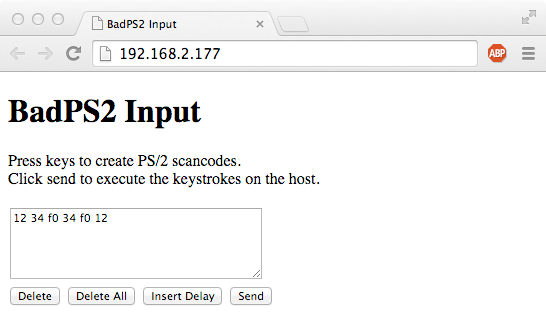
\includegraphics[width=1\textwidth]{images/website.jpg}
  \caption{Bildschirmfoto der Webseite}
  \label{website}
\end{figure}



\subsection{Gesamter Programmablauf}
Innerhalb dieses Teilabschnitts wird der gesamte Programmablauf betrachtet. Zu Beginn der Implementierung werden die benötigten Bibliotheken SPI für die Konsole, Ethernet für den Netzwerkanschluss und SD für den SD-Karten-Anschluss eingebunden \cite{arduino_libraries}. Anschließend werden benötigte Variablen deklariert, die in den hier dokumentierten Methoden Anwendung finden. Dazu zählen die Pinnummern für die Daten- und Taktleitung jeweils für den PS/2 Male und Female Anschluss, die Pinnummer für die SD-Karte und die drei Funktionalitäten. Zudem wird der Dateiname auf der SD-Karte mit ``data.txt'' festgelegt, in welchem einerseits die Tastatureingaben gespeichert werden und andererseits zur Wiedergabe verwendet werden. Weiterhin wird die MAC- und IP-Adresse des Mikrocontrollers und der Webserver auf Port 80 festgelegt, sowie ein String als Buffer deklariert.

Mithilfe der beiden Arduino Standardmethoden void setup() und void loop() werden dann die benötigten Komponenten initialisiert und der Programmablauf gestartet \cite{arduino_language}. In den folgenden Teilabschnitten wird die genaue Implementierung dieser beiden Methoden beschrieben und die Implementierung der Methoden, welche die einzelnen Funktionalitäten starten.

\subsubsection{void setup()}
Dies ist eine Standardmethode des Arduino Mikrocontrollers, welche einmalig aufgerufen wird, sobald der Mikrocontroller Strom hat oder zurückgesetzt wird \cite{arduino_language}. Damit besteht z.B. die Möglichkeit der Initialisierung verschiedener Komponenten, die mit dem Mikrocontroller kommunizieren. In diesem Fall werden zuerst die Pins initialisiert, über welche die drei Funktionalitäten ausgewählt werden können. Nach 1 Sekunde Verzögerung wird die Ausgabekonsole initialisiert. Anschließend werden die Methoden initKeys(int dataPin, int clockPin) und initCard(int sdPin) aufgerufen, zur Initialisierung der Tastatur und SD-Karte. Zudem wird auch der Ethernet-Anschluss des Mikrocontrollers initialisiert und der Webserver gestartet.

\subsubsection{void loop()}
Bei dieser Methode handelt es sich ebenfalls um eine Standardmethode des Arduino Mikrocontrollers, die nach jedem Durchlauf immer wieder erneut aufgerufen wird, sodass eine Interaktion möglich ist \cite{arduino_language}. Innerhalb eines Durchlaufs wird überprüft, ob einer der Pins für die Funktionalitäten auf High gesetzt ist. Falls dies für die Funktionalität der Aufnahme von Tastatureingaben der Fall ist, wird die Methode void reader(char* filename) mit der zu Anfang festgelegte Variable filename aufgerufen. Falls der Pin für die Funktionalität der Wiedergabe von Tastatureingaben mittels SD-Karte auf High gesetzt ist, wird die Methode void writer(char* filename) mit der Variable filename aufgerufen, danach 1 Sekunde gewartet und die Methode void loop() komplett beendet. Dadurch wird der Wiedergabe nur einmalig ausgeführt und nicht andauernd. Für den Fall, dass der Pin für die Wiedergabe von Tastatureingaben über Ethernet auf High gesetzt ist, wird die Methode void sender() ausgeführt. Und schließlich wird für den Fall, dass keiner der Pins auf High gesetzt ist, eine entsprechende Notiz auf der Konsole ausgegeben und 1 Sekunde gewartet bevor die Schleife erneut beginnt.

\subsubsection{void reader(char* filename)}
Mithilfe dieser Methode werden die Tastatur-Eingabesequenzen eingelesen und in eine Datei abgespeichert. Als Parameter wird dieser Methode ein Dateiname übergeben, welcher für das Abspeichern verwendet wird. Zuerst wird mithilfe der Methode readKeys(int dataPin, int clockPin) und den Pinnummern des PS/2 Female Anschlusses die eingegebene Taste gelesen. Dann wird geprüft, ob das Lesen der Tasteneingabe ein Ergebnis zurückgegeben hat. Im Fall eines Ergebnisses wird diese eingegebene Taste an den Host mithilfe der Methode writeKeys(int dataPin, int clockPin, unsigned char data) und den Pinnummern des PS/2 Male Anschlusses gesendet. Weiterhin wird für das Abspeichern ein Leerzeichen hinter dem Scancode angehängt und ggf. vor dem Scancode eine Null, da diese bei der Formatierung zu einem String entfallen kann. Dann wird das Ergebnis einerseits auf der Konsole ausgegeben und andererseits durch die Methode writeFile(char* filename, String content) in die Datei auf der SD-Karte gespeichert. Falls das Lesen der Tasteneingabe nicht erfolgreich war, wird eine entsprechende Notiz auf der Konsole ausgegeben.

\subsubsection{void writer(char* filename)}
Diese Methode nimmt einen Dateinamen als Parameter entgegen und realisiert die Wiedergabe von Tastatur-Eingabesequenzen. Zu Beginn wird die Datei mit dem übergebenen Dateinamen durch die Methode readFile(char* filename) ausgelesen und die Ausgabe des Dateiinhalts auf der Konsole vorbereitet. Für das Formatieren und Senden der Tastatur-Eingabesequenzen wird der Inhalt an die Methode sender(String content, char* separator) mit einem Leerzeichen als Separator übergeben.

\subsubsection{void website(EthernetServer webServer)}
Diese Methode ermöglicht einerseits die Ausgabe der Webseite an einen Anwender, aber auch die von dort gesendeten Tastatureingaben werden entgegen genommen und an den Host gesendet. Zu Beginn wird ein möglicher Client angelegt und falls dieser existiert, wird eine Schleife durchlaufen solange der Client verbunden ist. Falls dieser Client zusätzlich noch verfügbar ist und eine Nachricht sendet, dann wird jeweils ein Zeichen pro Schleifendurchlauf vom Client empfangen und einem Puffer hinzugefügt. Anschließend wird geprüft, ob das letzte gesendete Zeichen ein Zeilenumbruch ist und in dem Puffer nicht das Wort ``favicon'' steht, sodass die Webseite selbst angefordert wurde. Dann wird die Webseite mithilfe der Methode sendWebsite(EthernetClient client) an den Client gesendet. Zusätzlich wird der Puffer nach der Variable ``scan'' durchsucht, die den Inhalt des Textfeldes von der Webseite überträgt. Die Werte dieser Variable werden separiert und durch die Methode sender(String content, char* separator) mit dem Trennzeichen ``+'' als Tastatureingaben an den Host gesendet. Schließlich wird die Schleife beendet, 1ms gewartet und die Verbindung zum Client getrennt.

\subsubsection{void sender(String content, char* separator)}
Dieser Methode werden Tastatureingaben als String mit einem Trennzeichen übergeben, sodass diese in einer Schleife getrennt werden. Dafür wird bei jedem Durchlauf die Stelle des nächsten Trennzeichens ermittelt. Falls noch ein Trennzeichen in dem String vorhanden ist, wird der String vom ersten bis zum Trennzeichen zu einem Hexadezimalwert umgewandelt und auf der Konsole ausgegeben. Weiterhin wird geprüft, ob dieses Zeichen 0x00 ist. Da dies ein eigens eingeführtes Verzögerungszeichen ist, um Pausen zwischen Tasteneingaben setzen zu können, wird in einem solchen Fall der Programmablauf um 2s verzögert. Andernfalls wird durch die Methode writeKeys(int dataPin, int clockPin, unsigned char data) die Tasteneingabe als Scancode an den Host gesendet. Schließlich wird am Ende eines Schleifendurchlaufs der bisher schon betrachtete Teil des eingegebenen Strings abgeschnitten.



\section{Aufbau der Elektronik}
Die zu der Implementierung gehörende Elektronik besteht aus dem Mikrocontroller Arduino Mega 2560 Board und dem Arduino Ethernet Shield \cite{arduino}. Zudem wurde ein PS/2 Male Kabel \cite{ps2male} und ein PS/2 Female Kabel \cite{ps2female} verwendet, welche an jeweils einem Ende offen sind, wie in den Abbildungen \ref{ps2_male} und \ref{ps2_female} dargestellt \cite{ps2_male} \cite{ps2_female}. Zu der Implementierung gehören außerdem eine beliebige microSD-Karte, ein Steckbrett und drei 1k$\Omega$ Widerstände und diverse Drähte.
\begin{figure}
  \centering
  \begin{minipage}{0.45\textwidth}
    \centering
    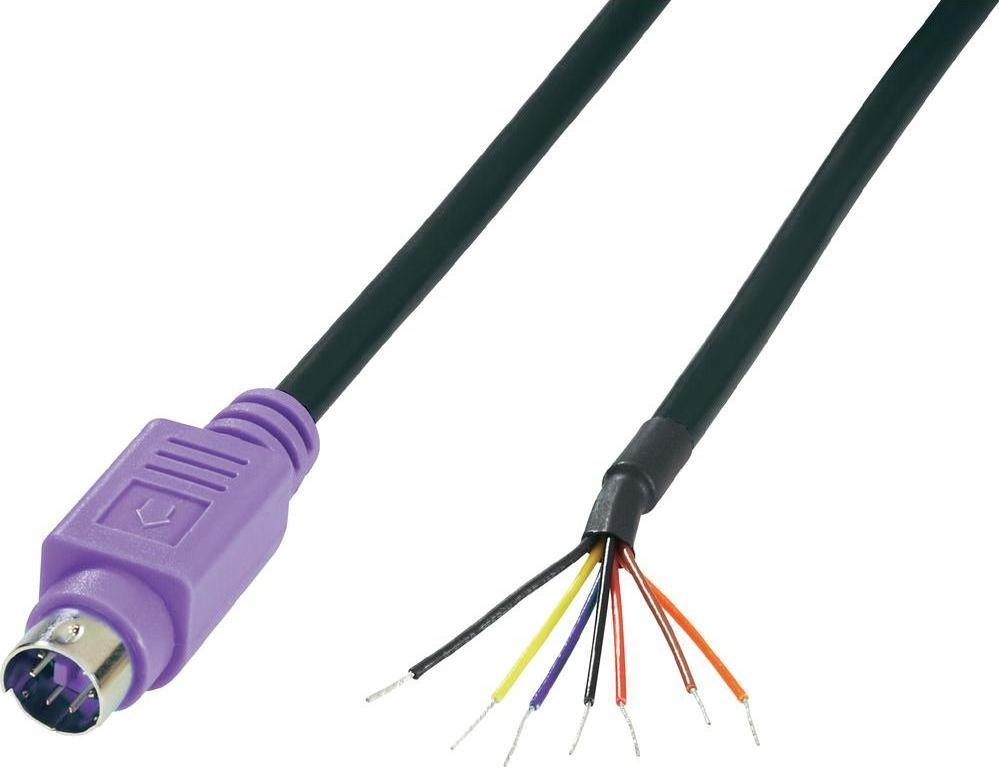
\includegraphics[width=1\textwidth]{images/ps2_male.jpg}
    \caption{PS/2 Male Kabel}
    \label{ps2_male}
  \end{minipage}
  \begin{minipage}{0.45\textwidth}
    \centering
    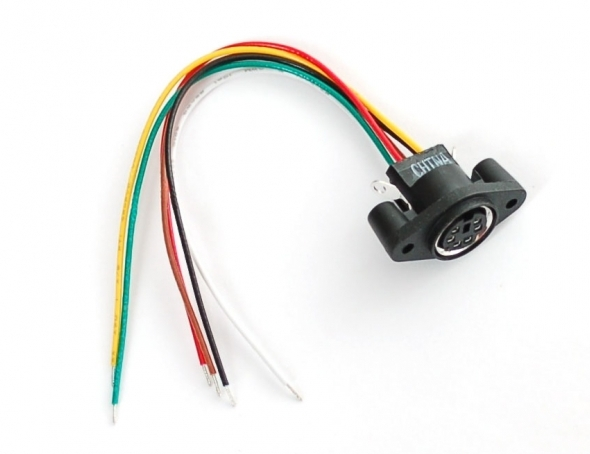
\includegraphics[width=1\textwidth]{images/ps2_female.jpg}
    \caption{PS/2 Female Kabel}
    \label{ps2_female}
  \end{minipage}
\end{figure}

Wie die Elektronik zusammengesetzt ist soll das Schema in Abbildung \ref{fritzing} verdeutlichen. Im linken oberen Teil des Schemas befinden sich die beiden PS/2-Kabel, der PS/2 Female Anschluss ganz links und rechts daneben der PS/2 Male Anschluss. Wie in den Grundlagen beschrieben, sind jeweils nur 4 Pins der Kabel in Benutzung, sodass auch nur 4 Kabel vom Steckbrett zum Mikrocontroller führen. Der Datenpin des Female Anschlusses führt über den grauen Draht zu Pin 2 des Mikrocontrollers und der Taktpin zu Pin 3. Für den PS/2 Male Anschluss sind dies jeweils Pin 18 und 19 für den Daten- und Taktpin.

Sowohl der 5 Volt Pin als auch der Pin für die Erdung werden über die violetten Drähte zusammengeführt und über die langen gelben Drähte auf die andere Seite des Mikrocontrollers geführt. Dort befinden sich ein 5 Volt Pin und ein Pin für die Erdung, welche über die grauen Drähte mit dem Steckbrett verbunden sind. Zudem existieren drei weitere Verbindungen von den digitalen Pins 44, 46 und 48 des Mikrocontrollers zum Steckbrett, worüber die drei implementierten Funktionalitäten ausgewählt werden können. Von der Erdung bestehen drei 1k$\Omega$ Widerstände jeweils zu den drei Leitungen der Funktionalitäten auf dem Steckbrett. Somit kann durch ein Umstecken des schwarzen Drahtes von der 5 Volt Verbindung zu den drei Verbindungen der Funktionalitäten jeweils eine angesteuert werden.
\begin{figure}
  \centering
  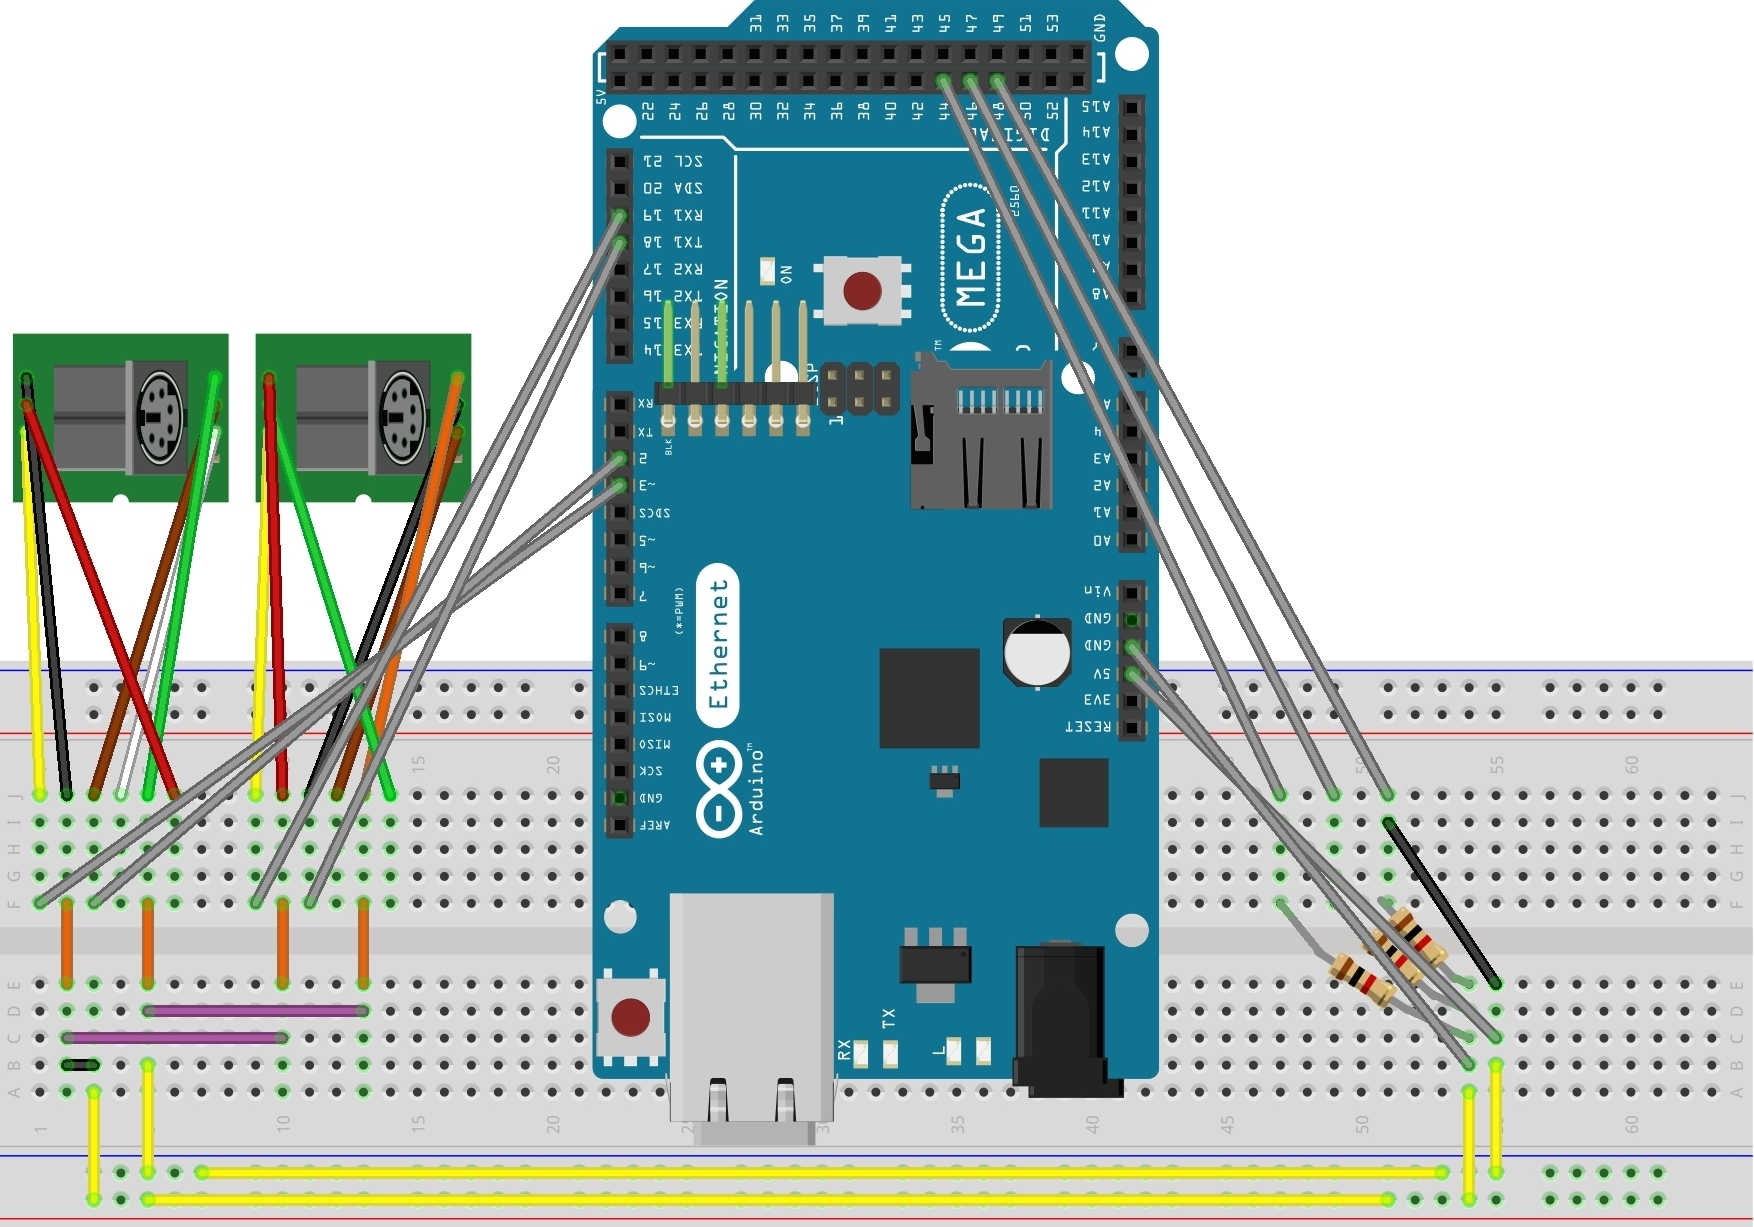
\includegraphics[width=1\textwidth]{images/fritzing.jpg}
  \caption{Fritzing-Schema der Elektronik}
  \label{fritzing}
\end{figure}

Das Foto in Abbildung \ref{foto1} zeigt abschließend die Implementierung. Die Mikrocontroller und die Kabel wurden mit Tesafilm auf dem Steckbrett fixiert, sodass die Implementierung transportiert werden kann.
\begin{figure}
  \centering
  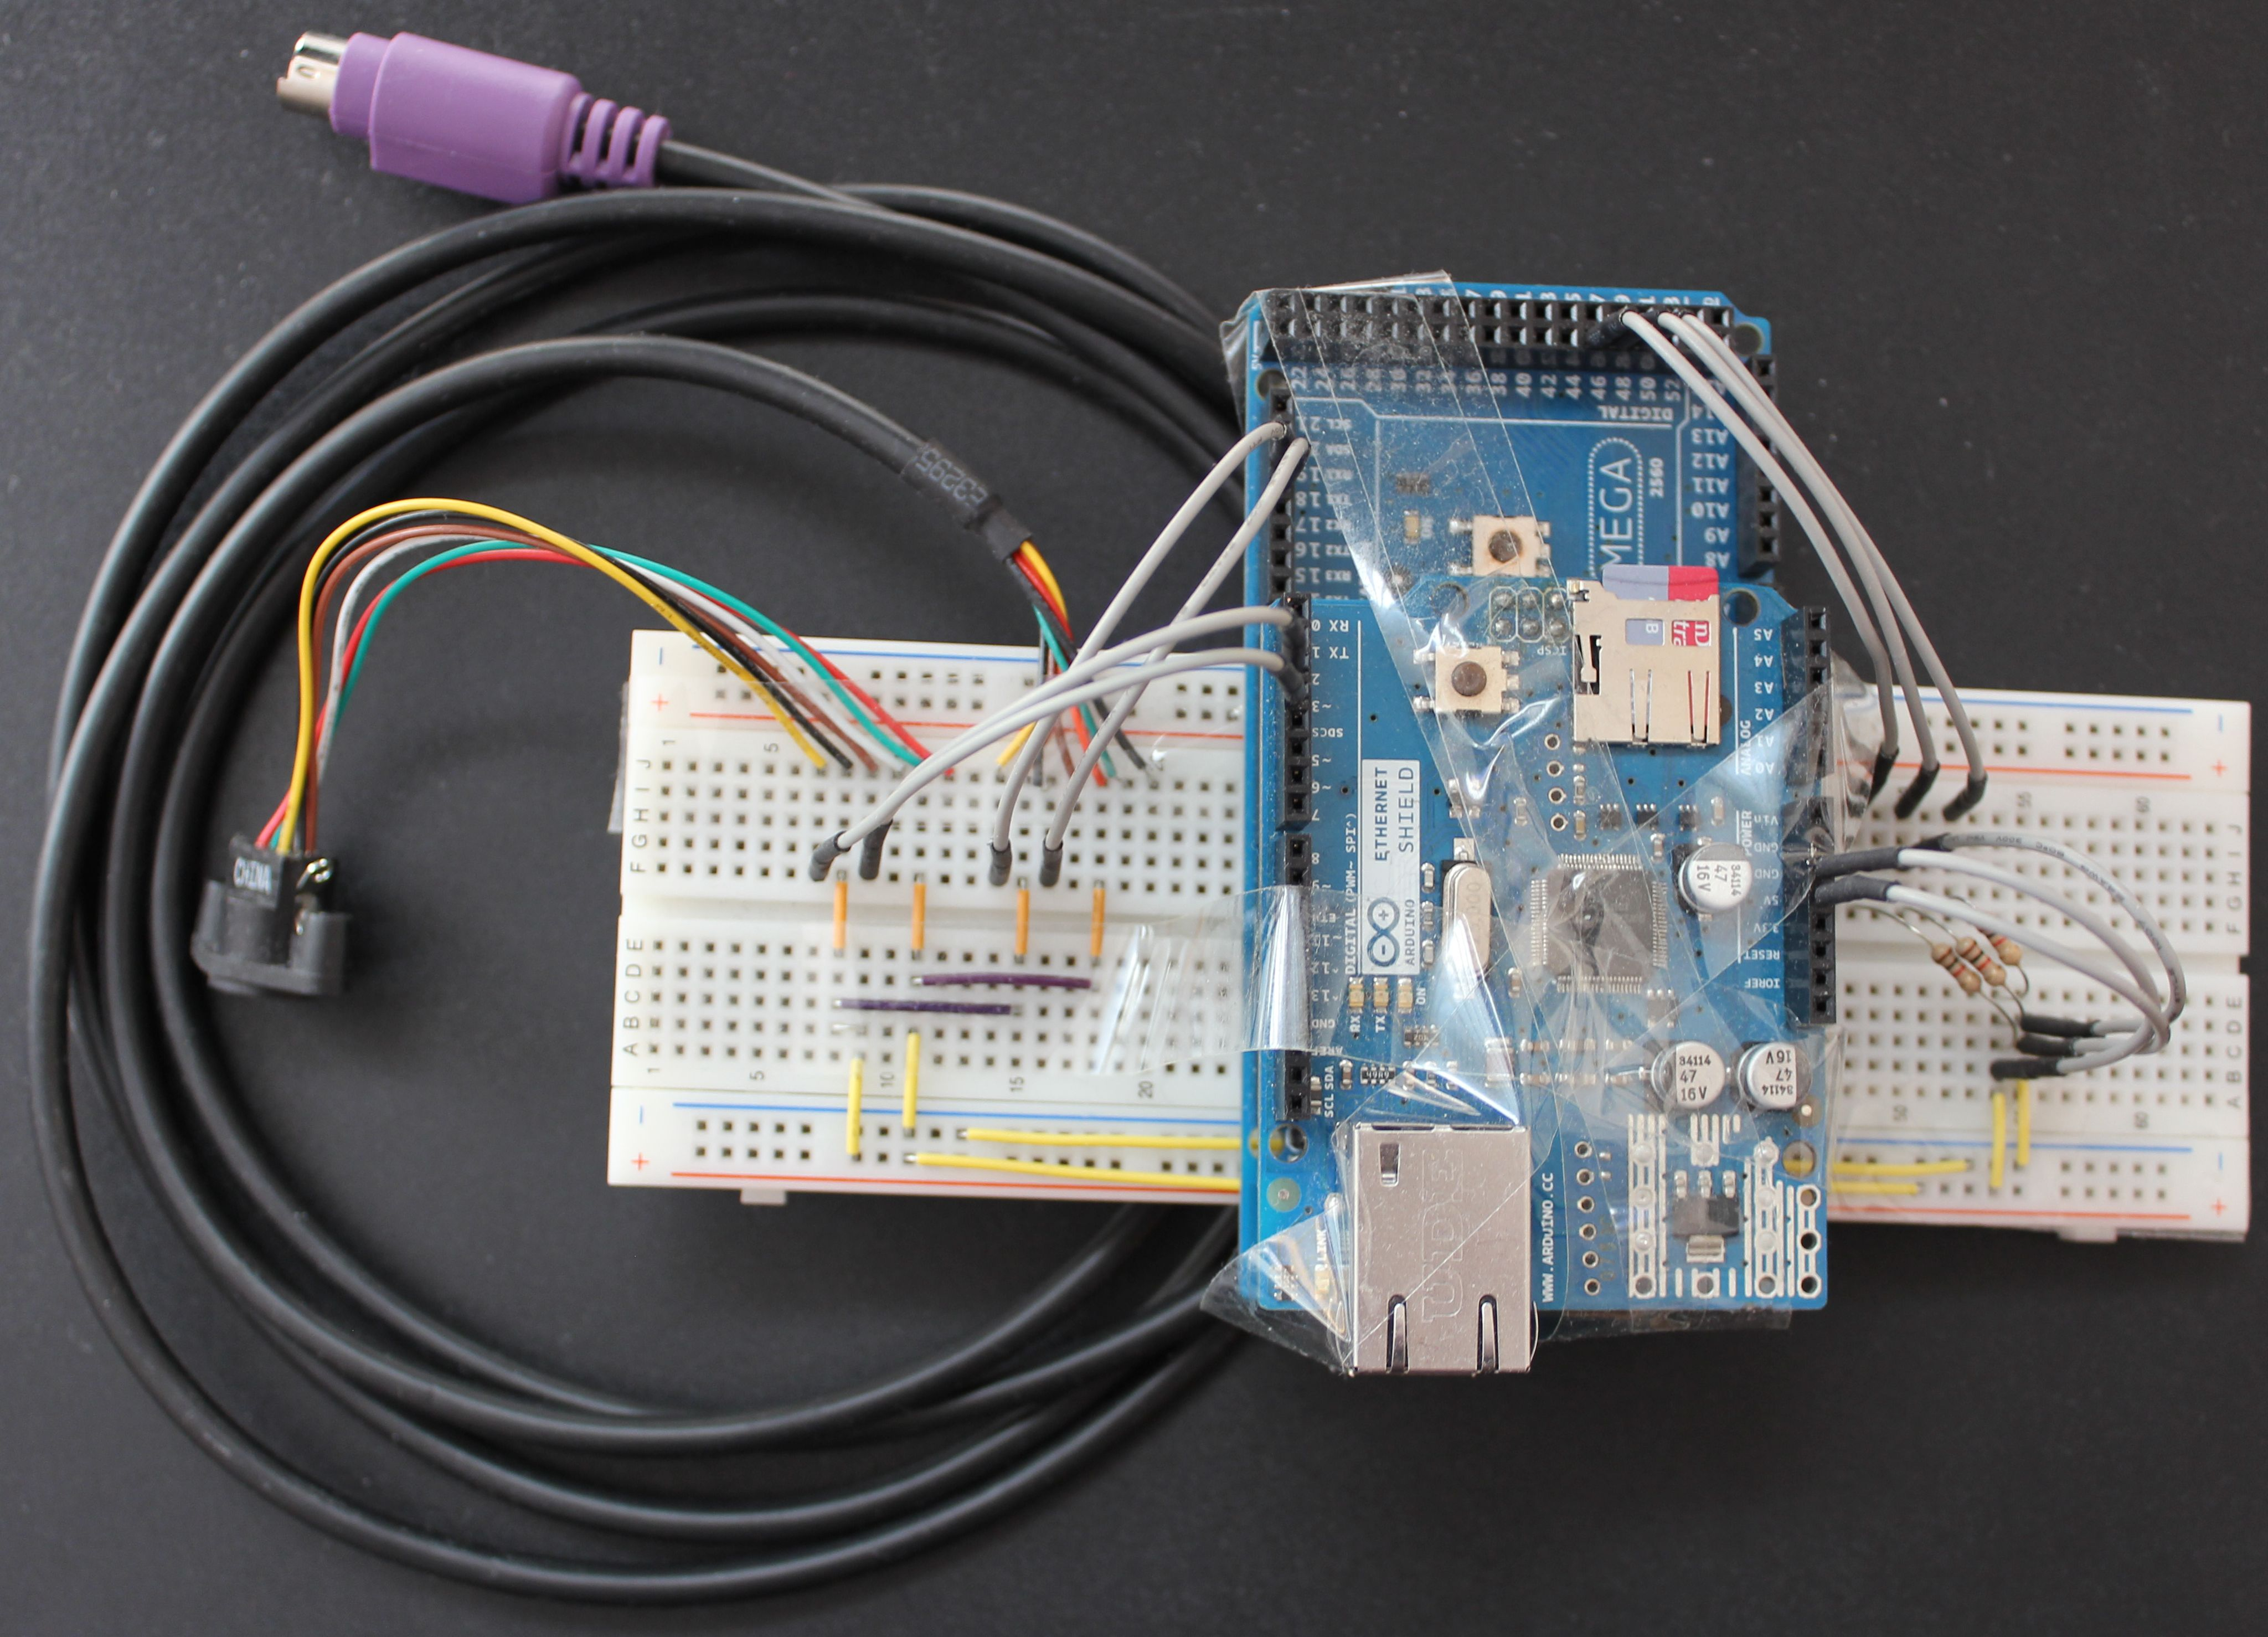
\includegraphics[width=1\textwidth]{images/foto1.jpg}
  \caption{Foto der implementierten Elektronik}
  \label{foto1}
\end{figure}